\subsection{Observer Effect and Telemetry Footprint Breakdown}

The empirical evaluation of monitoring overhead is crucial to ensure internal validity, as the instrumentation inherently perturbs the measured system---a phenomenon classically defined in computer science as the \textit{Observer Effect} \cite{jain_1991, gregg_2020}. In containerized microservice orchestrations, if the telemetry footprint is unbounded, the observability architecture itself can degrade into a \textit{Noisy Neighbor} \cite{krebs_2012}, competing for shared node resources (e.g., CPU caches and network I/O) and artificially inflating business transaction latency.

The net resource overhead measured in Scenario 2 comprises two distinct operational layers, isolating in-band observer perturbation from out-of-band noisy neighbor risks:

\begin{enumerate}
    \item \textbf{In-Band Observer Effect (In-Workload Telemetry):} Within the application namespace (\texttt{otel-demo}), the in-process OpenTelemetry SDKs introduce a computational perturbation of $+234.40\,\text{mCPU}$ ($+39.80\%$). This localized overhead stems from distributed trace context propagation, span lifecycle bookkeeping, and the asynchronous gRPC serialization of OTLP batches. Crucially, workload resident memory remained stable at $3{,}714.50\,\text{MiB}$, confirming that ring-buffer queuing implemented by the OTel SDKs successfully prevents unbounded memory accumulation, mitigating out-of-memory (OOM) risks.
    
    \item \textbf{Out-of-Band Telemetry Stack (Noisy Neighbor Mitigation):} The centralized storage and processing stack within the \texttt{monitoring} namespace (Grafana Tempo, Loki, Prometheus, Promtail, and the OpenTelemetry Collector) operates with a static footprint of $165.60 \pm 22.97\,\text{mCPU}$ and $2{,}598.63 \pm 2.50\,\text{MiB}$. By segregating these backend components into a dedicated namespace with explicit Kubernetes resource \texttt{limits} and \texttt{requests}, PANOPTES prevents the backend storage engines from monopolizing node CPU and acting as a noisy neighbor to the Astronomy Shop workload. In Scenario~2, this dedicated infrastructure accounts for only $16.75\%$ of the total active CPU and $41.16\%$ of total cluster resident memory, falling within acceptable bounds for enterprise observability clusters \cite{gregg_2020}.
\end{enumerate}

Figure~\ref{fig:scenario2_cpu_overhead} and Figure~\ref{fig:scenario2_memory_overhead} illustrate the respective distributions across the four observation dimensions.

\begin{figure}[htbp]
    \centering
    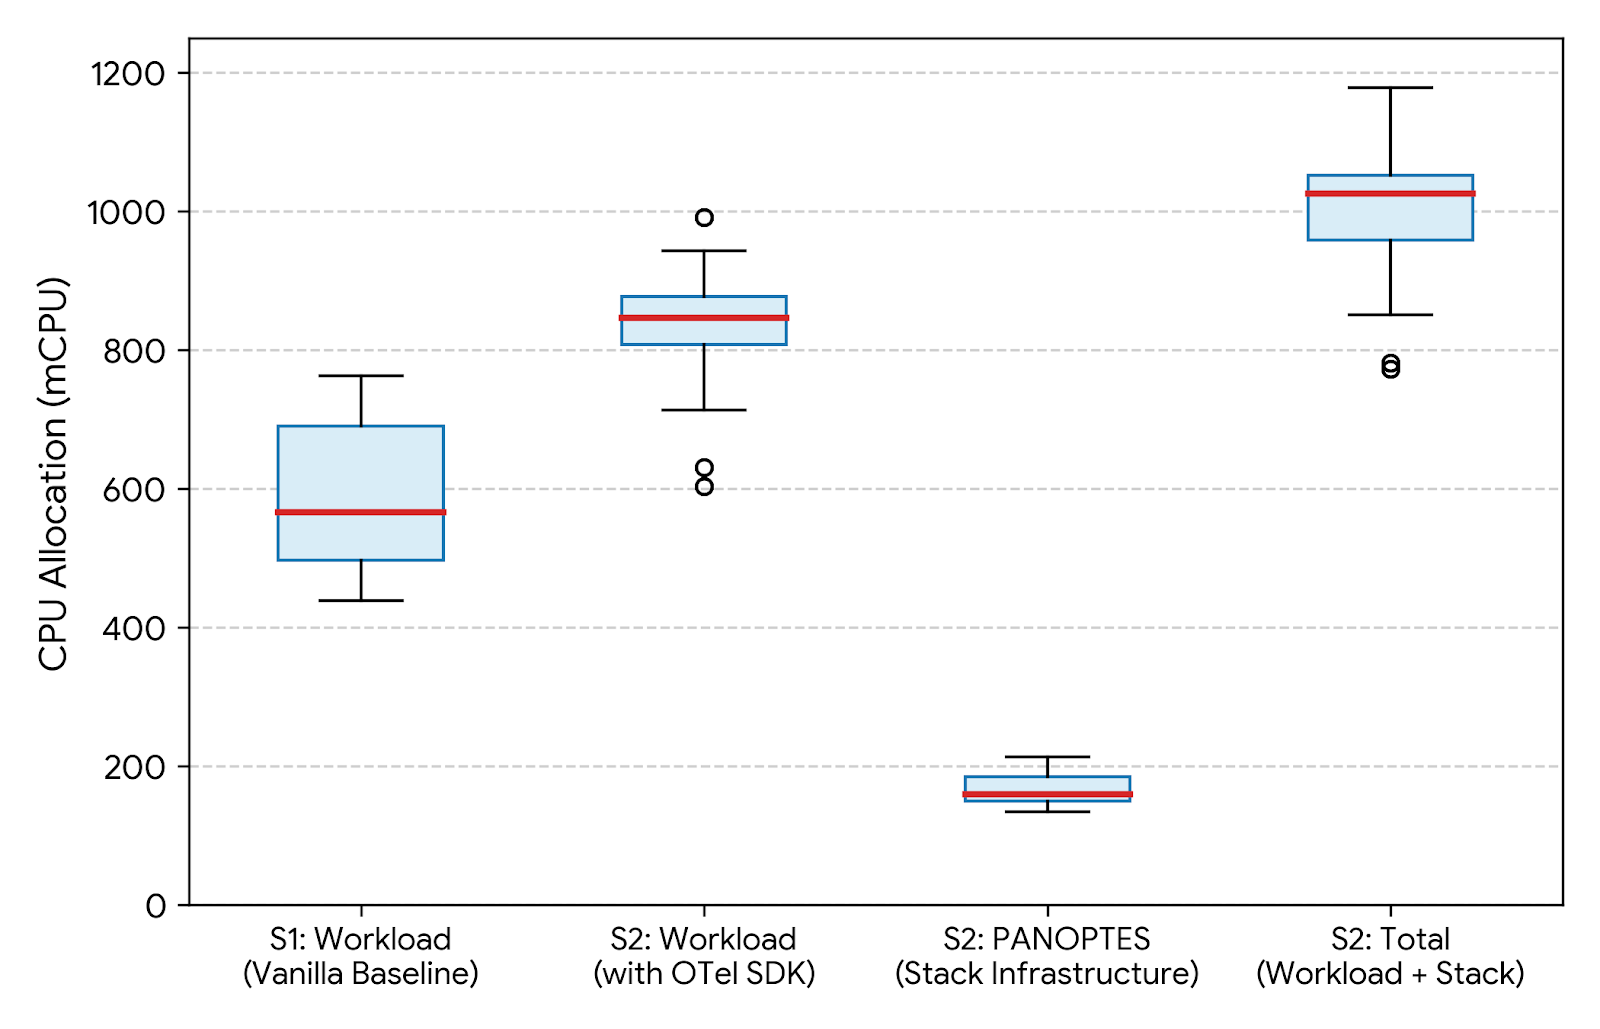
\includegraphics[width=0.75\textwidth]{images/results/scenario2_cpu_overhead.png}
    \caption{Steady-state CPU allocation distributions across Scenarios 1 and 2 ($N=30$).}
    \label{fig:scenario2_cpu_overhead}
\end{figure}

\begin{figure}[htbp]
    \centering
    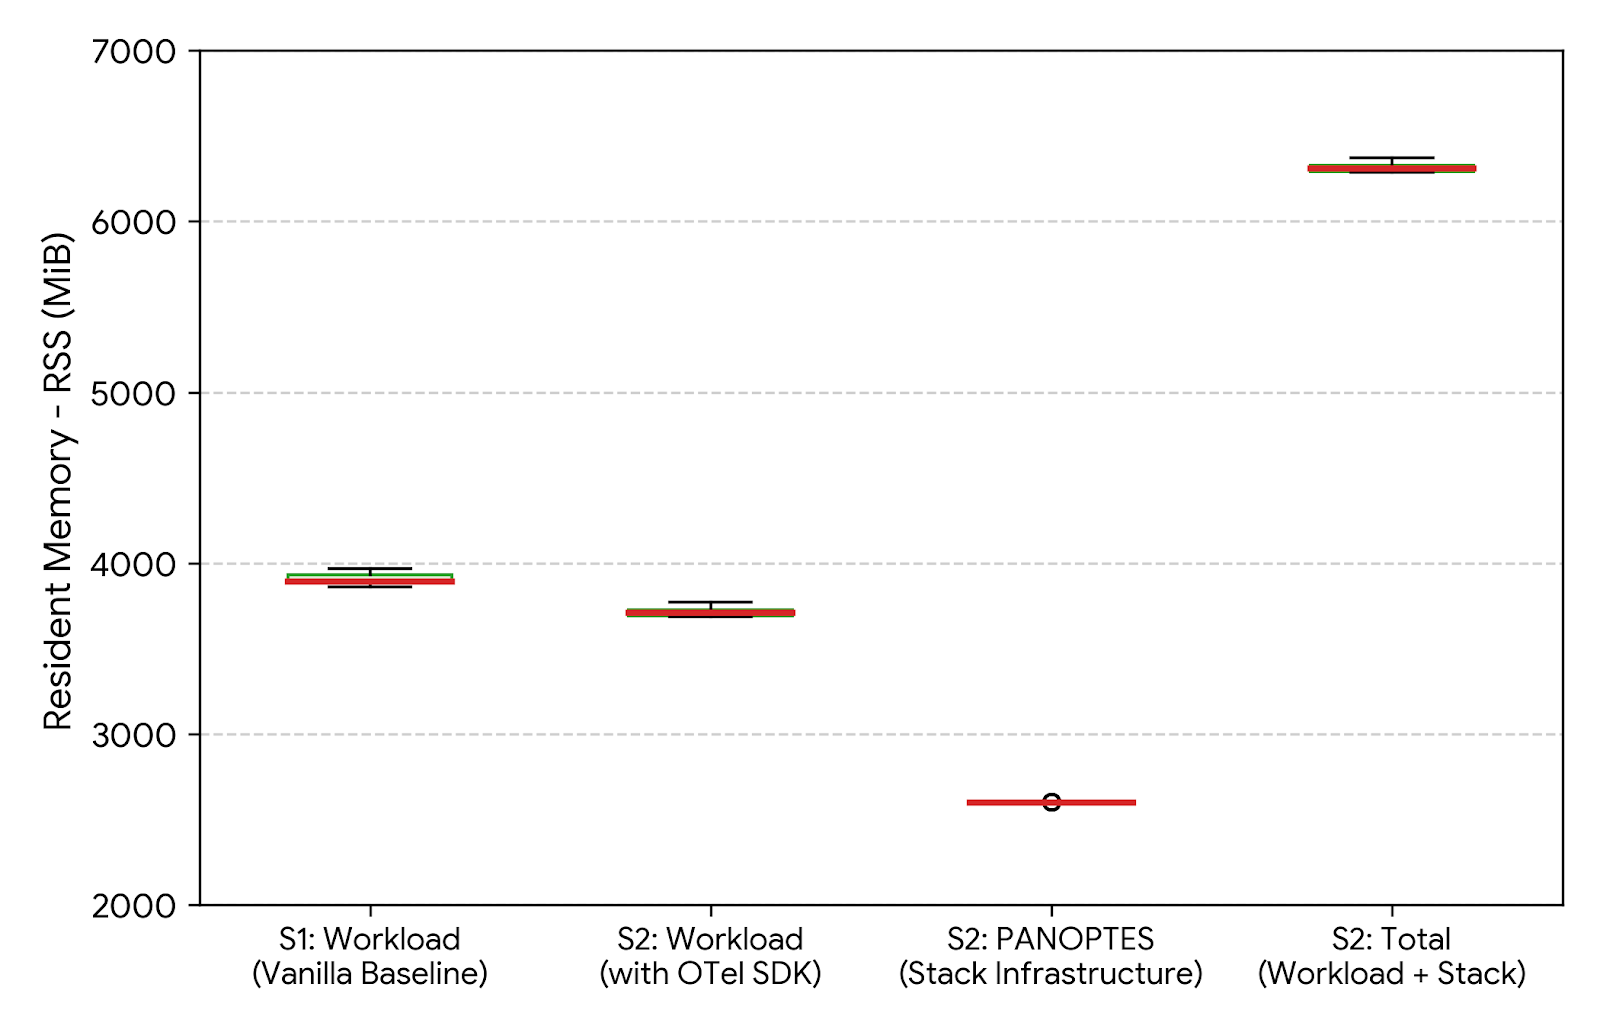
\includegraphics[width=0.75\textwidth]{images/results/scenario2_memory_overhead.png}
    \caption{Steady-state resident memory (RSS) distributions across Scenarios 1 and 2 ($N=30$).}
    \label{fig:scenario2_memory_overhead}
\end{figure}

A Shapiro-Wilk test confirmed non-normality across all metric distributions ($p < 0.05$). A two-sided Mann-Whitney $U$ test comparing total cluster demand between Scenario~1 and Scenario~2 confirmed statistically significant deltas for both CPU ($U = 0.0, \; p = 2.89 \times 10^{-11}$) and resident memory ($U = 0.0, \; p = 2.84 \times 10^{-11}$), validating the static baseline separation required to evaluate hypothesis $H_{1,3}$.